






\begin{figure*}
	\begin{center}

			\vspace*{-.35in}

	\begin{tabular}{  c c c  }
		%\hline
					\multicolumn{3}{c}{{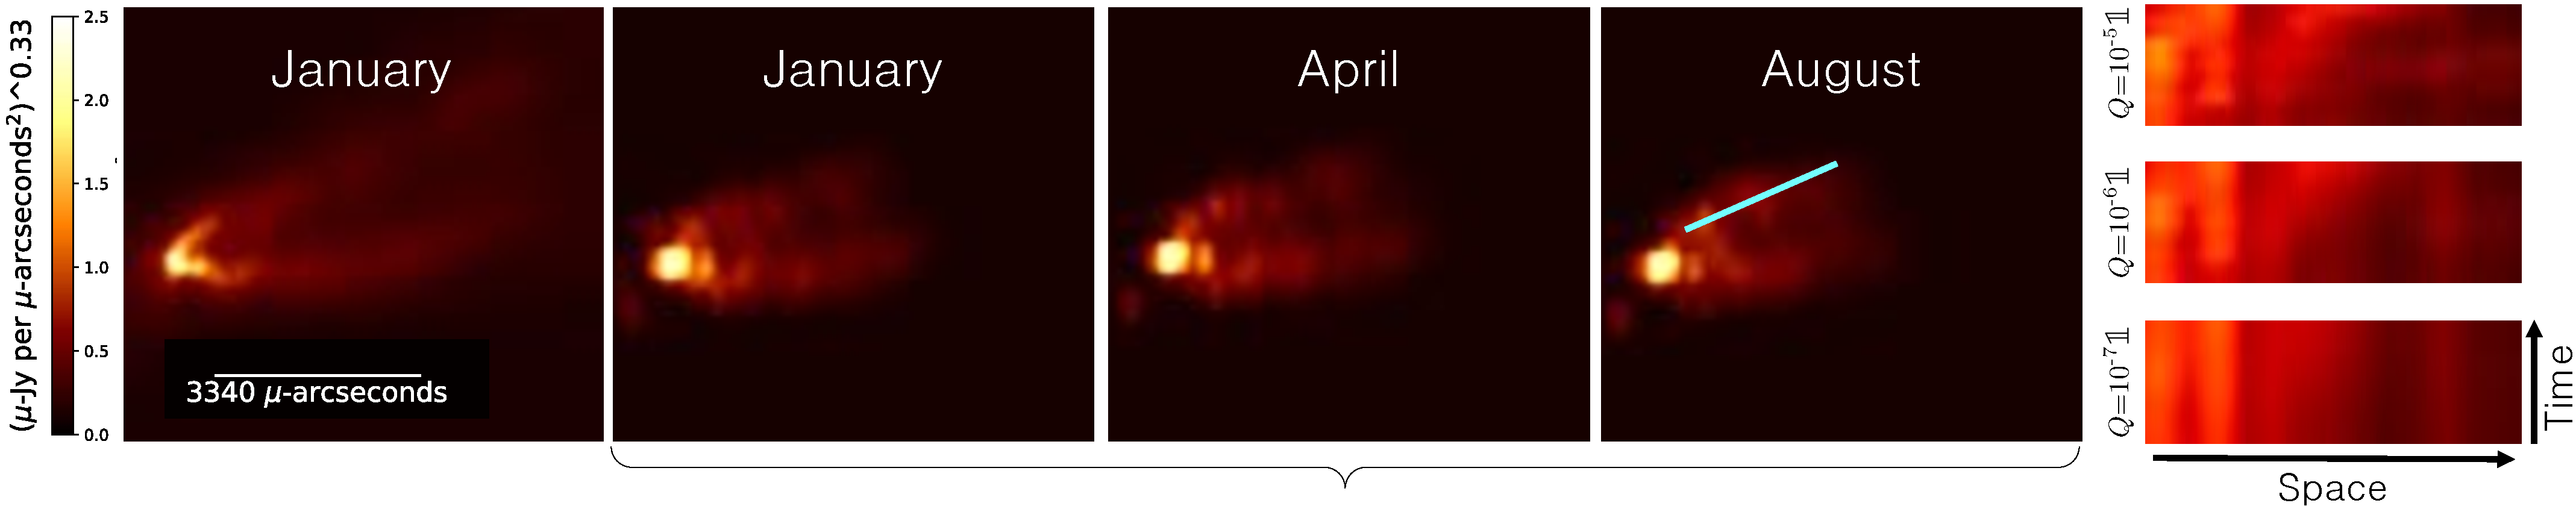
\includegraphics[width=1\linewidth]{figures/m87/m87_figure_r2.pdf}} } 
					\\
					\vspace{-.25in} && \\
%	\hspace{.8in}	\normalsize{\textsf{\cite{Johnson_dynamical} }}& \hspace{2.1in} \normalsize{\textsf{StarWarps }}&\hspace{1.5in} 	 \normalsize{\textsf{Space $\times$ Time Image }}\\
	\hspace{.8in}	\normalsize{\textsf{\cite{Johnson_dynamical} }}& \hspace{2.1in} \normalsize{\textsf{StarWarps }}&\hspace{1.5in} 	 \\
		\vspace{.1in} && 
\end{tabular}

\vspace*{-.27in}
		\caption{{\bf Video Reconstruction of Real Observations:} A StarWarps movie reconstruction obtained using real VLBI data taken of the M87 jet over the course of a year. Frames are shown with a gamma correction of $\gamma={1}/{3}$ to highlight weak emission. Data was collected in 2007 using the Very Long Baseline Array (VLBA) at 43 GHz~\cite{walker2016observations}. As the source structure does not evolve over the course of a night, traditional imaging approaches can be used to reconstruct `snapshot' images from this data. 
			The forked structure appearing in the StarWarps reconstructions also appears in images reconstructed using the CLEAN static imaging approach~\cite{walker2016observations} and the dynamic imaging approach presented in~\cite{Johnson_dynamical} (see left-most image). 
StarWarps produces a video that allows us to easily visualize the moving arms of the jet; the reconstructed video appears to contain outward motion, with a brighter region propagating down the arms. By visualizing the same slice of each frame (indicated by the cyan line) it becomes easier to see this motion as a static image (see the 3 Space $\times$ Time images on the far right). Note the diagonal `line' shown in the top 2 of these Space $\times$ Time images indicates a bright region moves down the arm, towards the right of the image. The intensity of these slices has been increased by $70 \%$ to highlight the evolving, weak emission. By controlling the amount of temporal regularization, $\bQ$, we control the amount of motion that appears in the reconstructed video. Increasing the temporal regularization, by decreasing $\bQ$, results in a Space $\times$ Time slice that varies less with Time. Individual frames shown were generated using $\bQ = 10^{\text{-}6} \mathds{1}$. }
\vspace{-.3in}
		\label{fig:m87}
	\end{center}
\end{figure*}



